\documentclass[a4paper]{article}

\usepackage[a4paper, margin=0.5in]{geometry}
\usepackage{graphicx}
\usepackage[linesnumbered,ruled,vlined]{algorithm2e}
\usepackage{color,soul}
\usepackage[utf8]{inputenc}
\usepackage[T1]{fontenc}
\usepackage{textcomp}
\usepackage{amsmath, amssymb}
\usepackage{caption}
\usepackage{listings}
\usepackage[italian]{babel}

% figure support
\usepackage{tikz}
\usetikzlibrary{calc}
\usepackage{import}
\usepackage{xifthen}
\pdfminorversion=7
\usepackage{pdfpages}
\usepackage{transparent}
\usepackage[hidelinks]{hyperref}
\usepackage{multirow}

\pdfsuppresswarningpagegroup=1

\begin{document}
	\title{Project log - Robotica}
	\author{Augello Andrea \and Castiglione Francesco Paolo \and La Martina Marco}
	\maketitle
	\tableofcontents

	\section{Setup}\label{sec:Setup}
	\begin{tabular}{|l|r|}
		\hline
		\multirow{2}{4em}{OS} & Ubuntu 18.04 \\
							  & Ubuntu 20.04 \\ \hline
		\multirow{2}{6em}{ROS version} & melodic \\
									   & noetic \\ \hline
		Webots & R2020b revision 1\\ \hline
		\multirow{2}{11em}{Target hardware} & Raspberry Pi 4B \\
											& Raspberry Pi 3B+ \\ \hline
	\end{tabular}

	\section{Nome}\label{sec:Name}
	Il team ha scelto il nome \textbf{Change} in onore di \textbf{Chang'e 4} \cite{change4}, la missione parte della seconda fase del programma cinese di esplorazione lunare, durante il quale è andato a buon fine il primo atterraggio morbido sulla faccia nascosta della luna. 

	\section{Ambiente}\label{sec:Libraries}
	Abbiamo considerato opportuno analizzare e studiare il package \textbf{webots\_ros} \cite{webotsRos} al fine di raggiungere una comprensione più profonda sulle metodologie per interfacciare i nodi ROS con il controller ROS standard per Webots. Inoltre è risultato necessario approfondire la documentazione ROS \cite{rosTutorial} al fine di installare e configurare l'ambiente ROS ed inoltre per capire i concetti fondamentali relativi ai nodi e topics. Infine abbiamo impostato l'interfaccia ROS su Webots seguendo la documentazione cyberbotics rilevante \cite{rosTutorial}.
	
	\section{Dipendenze}
	La seguente è una lista delle librerie utilizzate nel nostro progetto ed una breve spiegazione della loro funzione e rilevanza:
	
	\begin{itemize}
		\item opencv 4.x, una libreria per la computer vision, usata per operazioni di segmentazione \cite{opencv};
		\item imutils, che include funzioni per semplici operazioni di image processing quali traslazioni, rotazioni, ridimensionamento \cite{imutils};
		\item sklearn, una libreria per il machine learning comprendente algoritmi di clustering quali DBSCAN \cite{scikit};
		\item numpy, una libreria che fornisce supporto per array multidimensionali, matrici ed operazioni matematiche per lavorare su detti array \cite{numpy};
		\item matplotlib, una libreria per creare visualizzazioni di dati (statiche, dinamiche, interattive) \cite{matplotlib};
		\item math, una libreria che fornisce funzioni matematiche definite dallo standard C \cite{math}.
	\end{itemize}

	\section{Obbiettivo}
	L'obbiettivo del robot è di \textbf{evitare assembramenti in ambienti indoor}. \newline
	Nella dimostrazione presentata il nostro robot rileva le persone nella stanza e individua i possibili assembramenti. In seguito alla fase di rilevazione si sposterà verso l'assembramento evitando gli ostacoli e, arrivato, esorterà le persone al rispetto del distanziamento sociale.
	
	\section{Tiago Iron} 
	Il
	
	
	The robot selected for the given task is the \textbf{TIAGo Iron}. \newline\textbf{PAL Robotics TIAGo Iron}\cite{tiagoiron} is a two-wheeled human-like robot with a torso and a head but no articulated arm. The model is a modular mobile platform that allows human-robot interaction.\newline
	We added a \textbf{speaker} and a \textbf{display} with a corresponding support solid to the base TIAGo model available in Webots.
	We also had to ask the Webots developers for the precise size of the \textbf{wheels} since the model does not exactly match the specifications given in the data TIAGo datasheet\cite{Tiago IRON datasheet} and we discovered that they are 200mm.
	\newline We also decided to modify the IMU in order to best fit our goals and use an IMU with 6 degrees of freedom.
	The IMU consists of the following components:
		\begin{enumerate}
			\item gyro;	
			\item accelerometer;
		\end{enumerate}
	We decided to \textbf{not use the compass} because in a real scenario it would have been subject to various degrees of interference (significantly more so than a gyro), especially in an environment with many metal objects.
	
	\section{Positioning}
	In order to obtain the linear motion from the IMU a double integral is applied to the signal. The mathematical reasoning behind such approach is to remember that acceleration is the rate of change of the velocity of an object. At the same time, the velocity is the rate of change of the position of that same object. Since integration is the opposite of the derivative, if we know the object's acceleration we can get the position through double integration.
	
	\section{Projection Matrix}
	\cite{OpenGL}
	
	\section{Object recognition}
	We evalued performance between YOLO V3, TinyYOLO, HoG , HoG + SVG  , HoG + SVG + NMS. Yolo wins because it is 443\% more efficient. Width and not height. Yolo yields much tighter bounding boxes. 
	
	\section{Clustering}
	We decided to lower the dimensionality of our data. We used cylindrical coordinates and the feature vector is 2 dimensional.
	We used the Density-Based Scan with a threshold. The entities not belonging to the cluster are discarded.
	
	\section{ROS}
	
	\section{Bugs found in the Webots ROS Controller}
	Logical values did not allow callbacks.
	

	\section{Distance calculation}\label{sec:Distance-calculation}
	The perceived object height is not a reliable indicator of its distance
	since part of the object may be occluded or not present in the frame.
	Moreover, some classifiers like the HoG based ones tend to produce ROIs
	significantly taller than the object.
	
	The torso width, on the other hand, is less susceptible to these issues,
	and does not depend on the pose (e.g. sitting vs standing). We however need
	to assume a cylindrical torso, introducing some error if the target is not
	facing the camera.

	The horizontal position of the object relative to the camera can influence
	its perceived width, shrinking it the further it is from the center of the
	image.  Assuming that a camera has a FOV of $2\alpha$ and has a distance
	$d$ from the object, the maximum horizontal distance a point in the image
	can have from the center of the image plane is $a = d \tan alpha$
	(Fig.~\ref{fig:error}).

	\begin{figure}[htpb]
		\centering
		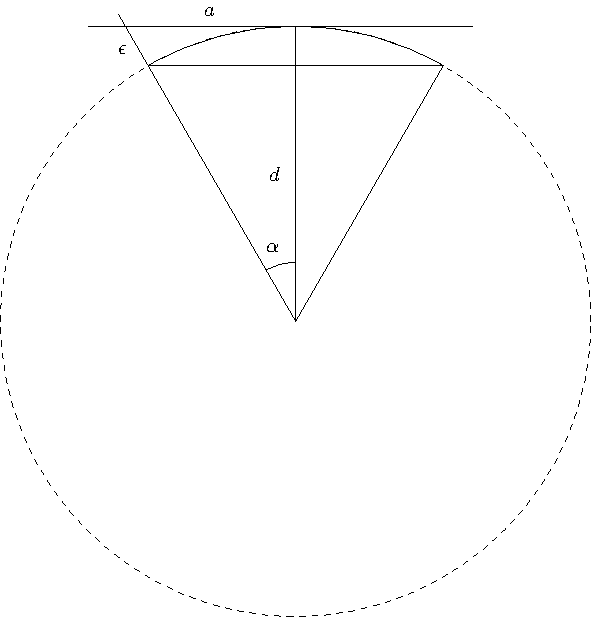
\includegraphics[width=0.8\textwidth]{./img/linearization_error.pdf}
		\caption{Error in distance estimate with piecewise circle linearization}
		\label{fig:error}
	\end{figure}

	Ignoring the perspective means performing a first order linear
	approximation and treating the point as if it lies in a circumference
	centered on the camera with $d$ as its radius. Hence, we consider the point
	being closer, committing the error shown in Eq.~\ref{eq:max_err}. With a
	camera FOV of 1 radiant as with the TIAGo this means that the maximum error
	due to the linearization amounts to a 13.9\% underestimate.

	\begin{equation}
		\epsilon = 
		\sqrt{a^2+d^2} - d =
		\sqrt{(d\tan \theta )^2+d^2}-d =
		d\left( \sqrt{\frac{1}{\cos ^2 \alpha}}-1 \right) =
		d \left( \sec \alpha -1 \right) 
		\label{eq:max_err}
	\end{equation}


	Under these assumptions we can compute the distance of an object as shown in
	Eq.~\ref{eq:obj_dist}

	\begin{equation}\label{eq:obj_dist}
		object~distance(m) = 
		\frac{f(m) \times real~width(m) \times image~width(pixels)}
			{object~width(pixels) \times sensor~width(m)}
	\end{equation}

	Since we are using a simulator, there is no camera sensor with a width to
	plug inside eq.~\ref{eq:obj_dist}. By placing both the robot and an object
	with known size in known positions and using this data together with pixel
	measurements in eq.~\ref{sensor_size}, we estimated the virtual sensor size
	to be used in all following computations.

	\begin{equation}\label{sensor_size}
		sensor~width(m) = 
		\frac{f(m) \times real~width(m) \times image~width(pixels)}
			{object~width(pixels) \times object~distance(m)}
	\end{equation}

	\newpage
	% Bibliography
	\bibliographystyle{unsrt}
	\begin{thebibliography}{19}
		\bibitem{tiagoiron} 
		\textit{https://cyberbotics.com/doc/guide/tiago-iron}. \newline
		Webots TIAGo Iron documentation.
		\bibitem{change4} 
		\textit{https://www.theguardian.com/science/2019/jan/03/china-probe-change-4-land-far-side-moon-basin-crater}. \newline
		The Guardian, 3 January 2019.
		\bibitem{webotsRos} 
		\textit{https://github.com/cyberbotics/webots\_ros}. \newline
		Github page for the \texttt{webots\_ros} package from \textit{cyberbotics}.
		\bibitem{rosTutorial} 
		\textit{https://wiki.ros.org/ROS/Tutorials}. \newline
		ROS documentation from ROS.org.
		\bibitem{webotsRosSetup} 
		\textit{https://www.cyberbotics.com/doc/guide/tutorial-8-using-ros}. \newline
		Cyberbotics documentation.
		\bibitem{Tiago IRON datasheet} 
		\textit{https://pal-robotics.com/wp-content/uploads/2019/07/Datasheet\_TIAGo\_Complete.pdf}. \newline
		Tiago IRON datasheet.
		\bibitem{OpenGL} 
		\textit{https://www.songho.ca/opengl/gl\_projectionmatrix.html}. \newline
		OpenGL Projection Matrix.
		\bibitem{positioning} 
		\textit{https://www.nxp.com/docs/en/application-note/AN3397.pdf}. \newline
		Implementing Positioning Algorithms Using Accelerometers.
		\bibitem{gmapping} 
		\textit{https://people.eecs.berkeley.edu/~pabbeel/cs287-fa11/slides/gmapping.pdf}. \newline
		Gmapping from UC Berkeley EECS, Pieter Abbeel.
		\bibitem{opencv} 
		\textit{https://opencv.org/}. \newline
		OpenCV Website.
		\bibitem{imutils} 
		\textit{https://github.com/jrosebr1/imutils}. \newline
		Imutils GitHub page.
		\bibitem{scikit} 
		\textit{https://scikit-learn.org/stable/}. \newline
		Scikit-learn website.
		\bibitem{numpy} 
		\textit{https://numpy.org/}. \newline
		Numpy website.
		\bibitem{matplotlib} 
		\textit{https://matplotlib.org/}. \newline
		Matplotlib website.
		\bibitem{math} 
		\textit{https://docs.python.org/3/library/math.html}. \newline
		Python documentation.
	\end{thebibliography}

\end{document}
